
Chcemy pokazać fajny algorytm zliczania wszystkich podziałów liczby $n$.

Oznaczmy liczbę wszystkich podziałów liczby $n$ jako $p(n)$. Jako ,,podziały liczby $n$'' mam na myśli liczbę sposobów na podzielenie liczby $n$ na ileś składników (niezerowych), np. liczbę $2$ mogę rozłożyć na $1 + 1$ albo po prostu na $2$ (i w sumie to tyle).  Funkcja tworząca ciągu $p_n$ to: \begin{equation*}
	P(x) = (1 + x + x^2 + x^3 + \dots) \cdot (1 + x^2 + x^4 + x^6 + \dots) \cdot (1 + x^3 + x^6 + x^9 + \dots) \dots
\end{equation*}

Pierwszy nawias odpowiada wybraniu jedynki do podziału (i temu ile razy ją bierzemy), drugi dwójki, trzeci trójki, etc.

Oczywiście przy $x^n$ będziemy mieli $p_n$, jak to działa w funkcjach tworzących (i mam nadzieję, że widać dlaczego). Zapisujemy $P(x)$ w fajniejszej postaci:

\begin{equation*}
	P(x) = \frac{1}{1-x} \cdot \frac{1}{1 - x^2} \cdot \frac{1}{1-x^3} \dots
\end{equation*}

Definiuję sobie $Q(x) = (1-x) \cdot (1-x^2) \cdot (1-x^3) \dots$. Zauważam, że $P(x) \cdot Q(x) = 1$, czyli $Q(x)$ jest funkcją odwrotną do $P(x)$. Okazuje się teraz, że $Q(x)$ jest funkcją tworzącą pewnego śmiesznego ciągu, który sobie zaraz pokażemy.

Póki co musimy wprowadzić oznaczenia:
\begin{enumerate}
	\item $e_n$ jest to liczba podziałów liczby $n$ na parzystą liczbę składników parami różnych,
	\item $o_n$ jest to liczba podziałów liczby $n$ na nieparzystą liczbę składników parami różnych.
\end{enumerate}
Jak wszyscy powinniśmy już wiedzieć, funkcja tworząca ciągu $e_n + o_n$ (czyli po prostu wszystkich podziałów $n$ ze składnikami parami różnymi) wygląda tak:
\begin{equation*}
	(1+x) \cdot (1 + x^2) \cdot (1+x^3) \dots
\end{equation*}
Ten fakt do niczego nam się w sumie nie przyda, ale może pomóc zrozumieć co zaraz się stanie.

Możemy sobie teraz podumać, jaka jest funkcja tworząca ciągu $e_n - o_n$. Otóż pojawia się tu plot twist, bo funkcja tworząca tego ciągu to po prostu $Q(x)$:
\begin{equation*}
	(1-x) \cdot (1-x^2) \cdot (1-x^3) \dots
\end{equation*}

Działa to tak jak w powyższym przykładzie, z tym że jeśli wybraliśmy nieparzyście wiele składników to będzie nieparzyście wiele minusów i się ,,odejmie'' od współczynnika przy $x^n$, a jeśli będzie parzyście wiele to się ,,doda''. Innymi słowy, do współczynnika przy $x^n$ doda się 1 za każdy możliwy podział na parzyście wiele parami różnych składników, a odejmie się 1 za każdy możliwy podział na nieparzyście wiele parami różnych składników, czyli to co chcemy. Nie do końca mam pomysł jak to formalnie wytłumaczyć, więc proszę użyć swojej intuicji™.

Po co to wszystko? Okazuje się, że ciąg $q_n = e_n - o_n$ ma pewne śmieszne własności (które niestety będzie trzeba udowodnić, brace yourselves).

\begin{theorem}[Eulera]
	\begin{equation}
		q_n = \begin{cases}
			0, \hspace{5pt} \mathrm{gdy} \hspace{5pt} n \not = \frac{(3 \cdot k \pm 1) \cdot k }{2} \\
			(-1)^k \hspace{5pt} \mathrm{wpp.}                                                       \\
		\end{cases}
	\end{equation}

\end{theorem}

\begin{proof}
	Zrobimy sobie przekształcenie $f$, które przesyła prawie (dlaczego prawie to dojdziemy do tego za chwilę) każdy podział na $n$ składników parami różnych na inny podział na $n$ składników parami różnych (bijektywnie). Ktoś powie że sobie zrobiłem świetną bijekcję idącą z pewnego zbioru w samego siebie, but hear me out: ta bijekcja będzie mieć tę śmieszną własność, że jeśli podział był na parzyście wiele składników to będzie przesłany na nieparzyście wiele, a jeśli na nieparzyście wiele to będzie przesłany na parzyście wiele składników. To będzie fajne, bo pokażemy sobie że jest ich tyle samo (poza przypadkami gdzie definicja tej funkcji się popsuje, ale o tym za chwilę).

	Generalnie to oznaczmy sobie najmniejszy składnik w podziale $P$ jako $a$. Ponadto, zdefiniujmy sobie zbiór $X$, taki że zawiera on największe składniki podziału $P$, takie że każde dwa sąsiednie różnią się o jeden. Innymi słowy, jeśli podział $P = (\lambda_1, \lambda_2, \lambda_3, \dots, \lambda_k)$, to $X =\{\lambda_1, \lambda_2, \lambda_3, \dots, \lambda_d\}$, gdzie $d$ jest największą liczbą taką, że kolejne składniki różnią się o 1  (zakładamy, że $\lambda_1 > \lambda_2 > \dots > \lambda_k$).

	Teraz jak mamy te zbiory zdefiniowane to możemy robić śmieszne rzeczy. Jeśli $|X| < a - 1$, to możemy przerobić nasz podział, odejmując od każdego elementu z $X$ 1, i dorzucając nowy element do podziału, taki że równy jest on moc $|X|$. Otrzymaliśmy oczywiście poprawny podział (niektórym może pomóc dowód przez rysowanie).

	Dlaczego $|X| < a - 1$, a nie po prostu $|X| < a$? Otóż przychodzi tutaj pewien śmieszny problem, mianowicie może być tak, że składnik podziału o wartości $a$ ,,wpadł'' do $X$. W takim przypadku bijekcja nam się kompletnie popsuje i wtedy jej definiujemy (ale jeszcze do tego wrócimy). Natomiast jeśli $a$ nie należy do $|X|$ to nasza bijekcja nadal działa. Fajnie.

	Czyli reasumując: jeśli $|X| < a - 1$ lub ($|X| = a - 1$ i $a \not \in X$) od każdego składnika z $|X|$ odejmujemy 1 i majstrujemy nowy składnik, który wrzucamy pod składnik o wartości $a$, który uprzednio był najmniejszy.

	\begin{figure}[H]
		\centering
		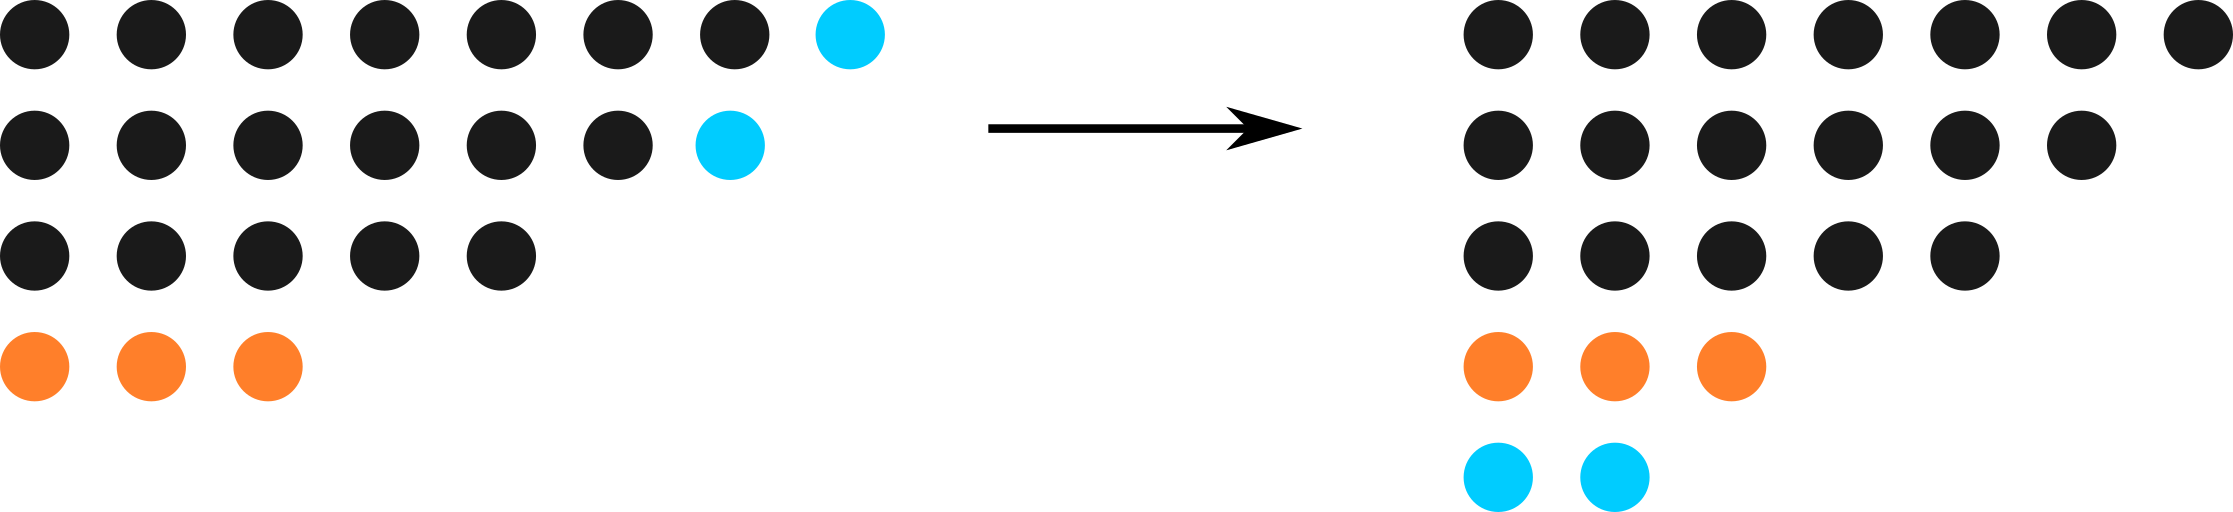
\includegraphics{images/case2.png}
		\caption{Wizualizacja przekształcenia (diagram Ferrersa). 2 ,,górne'' składniki różnią się o 1, trzeci już różni się od nich o 2; $|X| = 2$, $a=3$.}
	\end{figure}

	Zasadniczo to samo będziemy czynić (ale w drugą stronę), gdy okaże się że $a < |X| $. Ordynarnie \textit{wywalam} składnik $a$ i do odpowiedniej liczby elementów z $X$  ,,dodaję'' 1, tak by się wyrównało. Należy zauważyć, że być może nie wszystkie elementy z $X$ będą mieć coś do siebie dodane, ale to mi nic nie psuje. W sumie też fajnie byłoby dodać, że dodaję te jedynki najpierw największym składnikom; inaczej mogłoby to się popsuć.

	Co dzieje się, gdy $a = |X|$? Jeśli $a \in X$ to jest mi smutno, w przeciwnym razie mogę zrobić to samo co robiłem wcześniej i wszystko działa jak powinno.

	\begin{figure}[H]
		\centering
		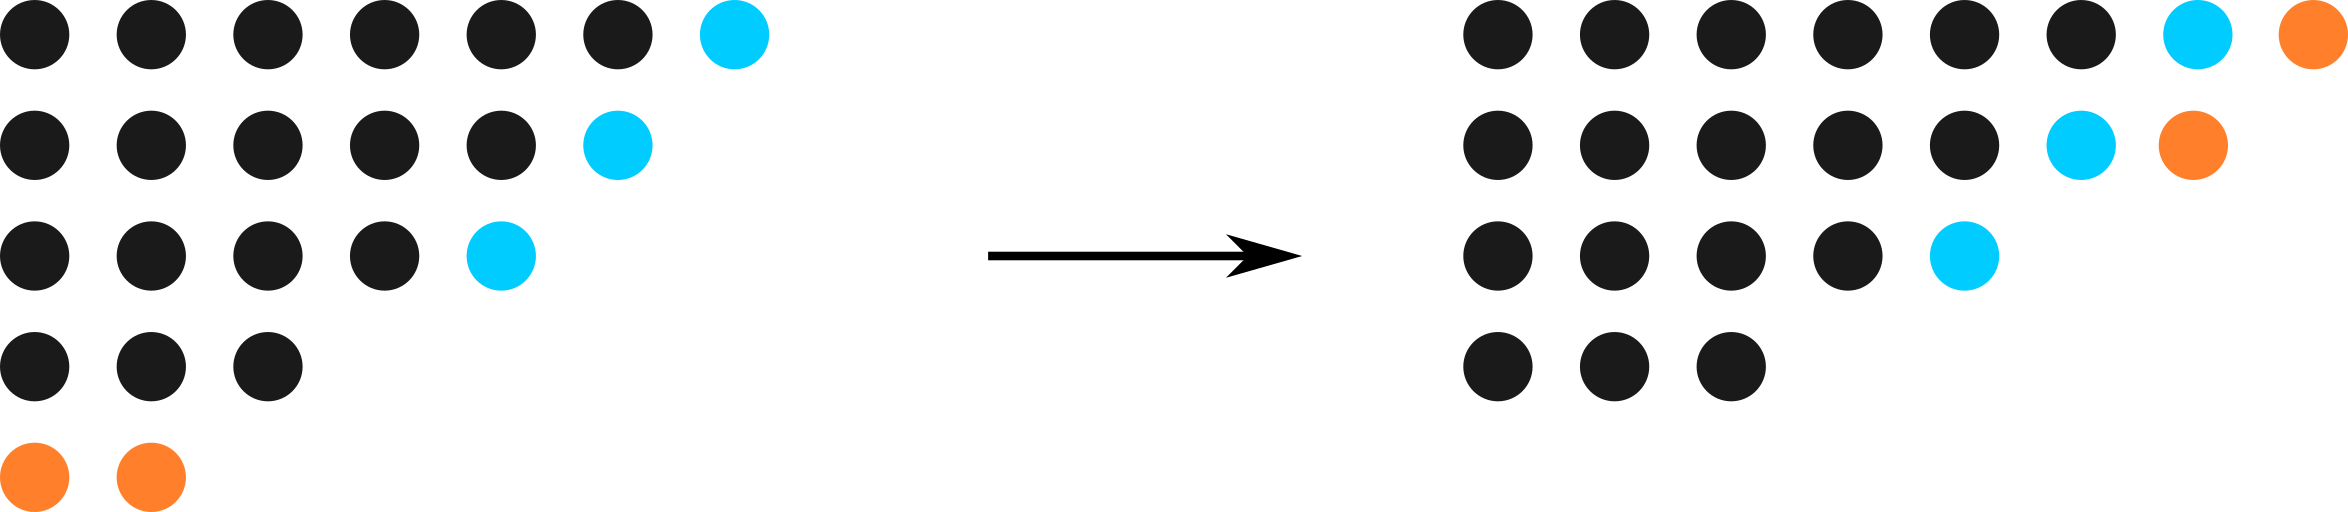
\includegraphics{images/case_1.png}
		\caption{Wizualizacja przekształcenia (diagram Ferrersa). 3 ,,górne'' składniki różnią się o 1 więc należą do $X$. $|X| = 3$, $a = 2$, więc dwóm największym elementom dodajemy 1, a składnik $a$ usuwamy.}
	\end{figure}

	Zostają więc 2 przypadki, gdy coś może się popsuć:
	\begin{enumerate}
		\item $|X| = a - 1$, $a \in X$
		      \begin{figure}[H]
			      \centering
			      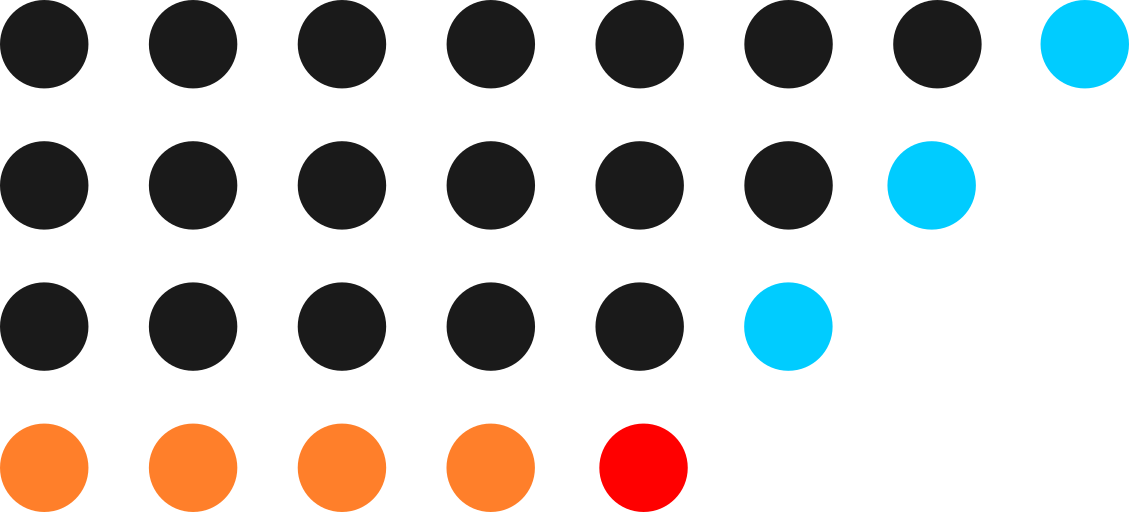
\includegraphics{images/irytujacy_1.png}
			      \caption{Gdy $|X| = a - 1$ i składnik $a$ jest w $X$; widać, że nic nie możemy z tym zrobić.}
		      \end{figure}

		\item $|X| = a$, $a \in x$
		      \begin{figure}[H]
			      \centering
			      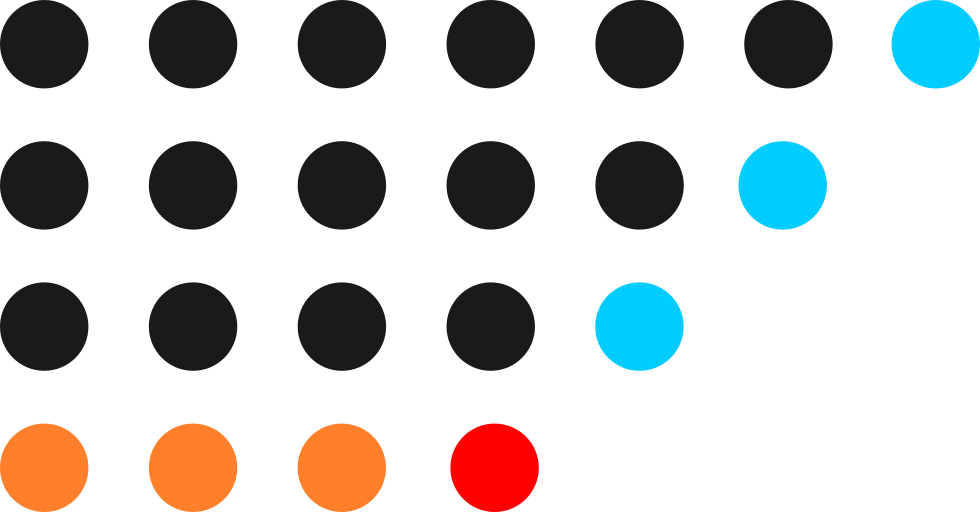
\includegraphics{images/irytujacy_2.png}
			      \caption{Gdy $|X| = a$ i składnik $a$ jest w $X$; również widać, że nasze przekształcenie nie zadziała.}
		      \end{figure}
	\end{enumerate}

	Zauważmy, że sytuacja gdy składnik $a$ jest w $X$ jest bardzo dziwną sytuacją generalnie, bo jest to najmniejszy składnik; z definicji $X$ mamy wtedy, że wszystkie kolejne składniki w $P$ różnią się o dokładnie 1. Na podstawie tej obserwacji możemy już dokładnie powiedzieć, jakiej postaci musi być $n$, by miało taki ,,złośliwy'' podział:

	\begin{enumerate}
		\item Gdy $|X| = a - 1$, $a \in X$, to $n$ musi dla jakiegoś $k$ być postaci $(k + 1) + (k + 2) + \dots + 2k $ ($|X| =k, a = k+1$, wszystko się zgadza)
		\item Gdy $|X| = a$, $a \in x$, to $n$ musi dla jakiegoś $k$ być postaci $k + (k+1) + (k+2) + \dots + (2k - 1)$ ($|X| = k$, $a = k$, ponownie wszystko gra)
	\end{enumerate}

	Jak zastosujemy matematykę mniej dyskretną by wysumować te nawiasy, dostaniemy że $n$ aby miało irytujący podział to musi być postaci $\frac{k \cdot (3k+1)}{2}$ lub ${k \cdot (3k-1)}{2}$. Jednocześnie nie ma takiego naturalnego $k$, że wartości te są sobie równe, więc jeśli $n$ ma irytujący podział, to ma go tylko jednego. Wtedy nie możemy przerzucić tylko jednego podziału na inny (inne są ze sobą w bijekcji) więc $e_n - o_n = (-1)^k$ (jeśli $k$ jest parzyste to irytujący podział ma parzyście wiele składników, a w przeciwnym razie nieparzyście wiele). Jeśli irytujący podział nie występuje, $e_n = o_n$ z bijekcji którą pokazaliśmy. Fajnie.
\end{proof}

Dobra, ale wróćmy do tego cośmy chcieli udowodnić na samym początku. Co w ogóle wynika z tego twierdzenia Eulera? No w sumie to bardzo dużo, bo jak mamy $q_n = e_n - o_n$ i $Q(x)$ jest jego funkcją tworzącą:
\begin{equation*}
	Q(x) = q_0 + q_1 \cdot x + q_2 \cdot x^2 + q_3 \cdot x^3 + \dots
\end{equation*}
Ale znamy wartości współczynników $q_i$ z twierdzenia Eulera:
\begin{equation*}
	Q(x) = 1 - x - x^2 + x^5 + x^7 - x^{12} - x^{15} + x^{22} + x^{26} + \dots
\end{equation*}
Zauważmy, że współczynników które nie są zerowe jest tylko jakoś $O(\sqrt{n})$, czyli dosyć mało.

Pamiętajmy, że $P(x) \cdot Q(x) = 1$, czyli że ciąg który wyjdzie po ich wymnożeniu będzie wyglądać tak: $(1,0,0,0, \dots)$ Ponieważ mnożenie w funkcjach tworzących działa jakoś tak, że w wynikowym ciągu (nazwijmy go $r$) element $r_n$ można obliczyć w ten sposób:
\begin{equation*}
	r_n = \sum_{i=0}^{n} p_n \cdot q_{n-i}
\end{equation*}

I wiemy że w naszym przypadku $r_n = 0$ dla $n > 1$, to mamy że: \begin{equation*}
	0 = p_n - p_{n-1} - p_{n-2} + p_{n-5} + p_{n-7} - p_{n-12} - \dots
\end{equation*}
To teraz $p_n$ przerzucamy na drugą stronę i mnożymy stronami razy $-1$ i mamy wzór na $p_n$, które możemy obliczyć w $O(\sqrt{n})$. No i fajnie.